\chapter{Lightweight Group-Key Management Scheme}
\label{ch:lightwightProto}
It is fundamental to ensure security in network services and applications of WSNs and efficient and lightweight key management has been identified as one of core mechanisms to solve this problem.
In multicast group communications, the energy consumption, bandwidth and processing overhead at the nodes are minimized compared to a point-to-point communication system \cite{Rahman2015}. 
The multicast communication protocol has to generate and distribute a secret group key that can be used to encrypt data sent from one source to all destinations that are member of the same group. 
Multicast groups are often very dynamic due to the join and leave of the members, and for this reason the protocol has to handle such group membership changes by re-generating and re-distributing new group keys in a secure and efficient matter. 

Group key management in WSN includes several processes and mechanisms to solve the problem of  establishing a secure links between the members of a group.
This includes establishing (or creating), distributing and maintaining secret keys \cite{He2013JournalSurvey}.
The key establishment techniques should guarantee the authenticity of all the sensor nodes involved in a particular communication and protect the disclosure of data to unauthorized parties (i.e., confidentiality) and from falsifications (i.e. integrity).

Depending on the ability to update the cryptographic keys of sensor nodes during their run time (re-keying), these schemes can be classified into two different categories: static and dynamic.  
In static key management, the principle of pre-shared key is adopted, and keys are fixed for the whole lifetime  of  the  network.  
However, the probability for a cryptographic key to be attacked increases significantly with the time.  
Instead, in dynamic key management, the cryptographic keys are refreshed  throughout the lifetime of the network.

The proposed protocol focuses on different problems related to group-key establishment and management.

First, is considered the problem of establishing a group shared secret among a group of end nodes. 
Then the author shows how a new node can be added to the group in such a way that the newly added node does not learn the previous group key or group communication. 
It is also shown how to remove a node from the group in such a way that it does not learn anything about the communications after it left the group. 
Finally, the problem of generating new session keys from the established group secret is analyzed.  

In this thesis, it has been adopted a slightly loose definition of forward and backward secrecy. 
By forward secrecy, the author means that an attacker will not able to learn future session keys or group communications even if the attacker managed to learn the current session key.
This also applies to which was a member of the group but that was later removed. 
Even that node had access to the session key when it was a member, it shall not be able to learn or derive session keys generated after it left the group. 
By backward secrecy, it is meant that a newly added node will not be able to learn previous session keys and/or group communication before it joined the group. 

\begin{table}[h]
\caption{List of Notations for the proposed scheme }
\label{notations}
\begin{center}
\begin{tabular}{|c||c|}
\hline
\textbf{Notation} & \textbf{Description}\\
\hline
\textit{G} & Gateway\\
\hline
$n_i$ & $i$th node\\
\hline
$k$ & number of nodes\\
\hline
$m$ & number of legitimate nodes\\
\hline
$PrivKey_i$ & $i$th node's private key\\
\hline
$PubKey$ & $i$th node's public key \\
\hline
$\mathbb{F}_q$ & finite field\\
\hline
$\mathbb{E}|\mathbb{F}_q$ & elliptic curve on the finite field $\mathbb{F}_q$\\
\hline
$s_i$ & secret shared between $i$th node and the gateway \\
\hline
E & generic symmetric encryption/decryption function (i.e, AES) \\
\hline
$MSK$ & final group shared secret (Master Shared Key) \\
\hline
$PRF$ & Pseudo Random Function \\
\hline
\end{tabular}
\end{center}
\end{table}

\section{Initialization Procedure}

\tikzstyle{drawrect}=[draw, rectangle,anchor=east, minimum height=8,
  minimum width=142pt,fill=Turquoise!20]
\begin{figure*}
\begin{center}
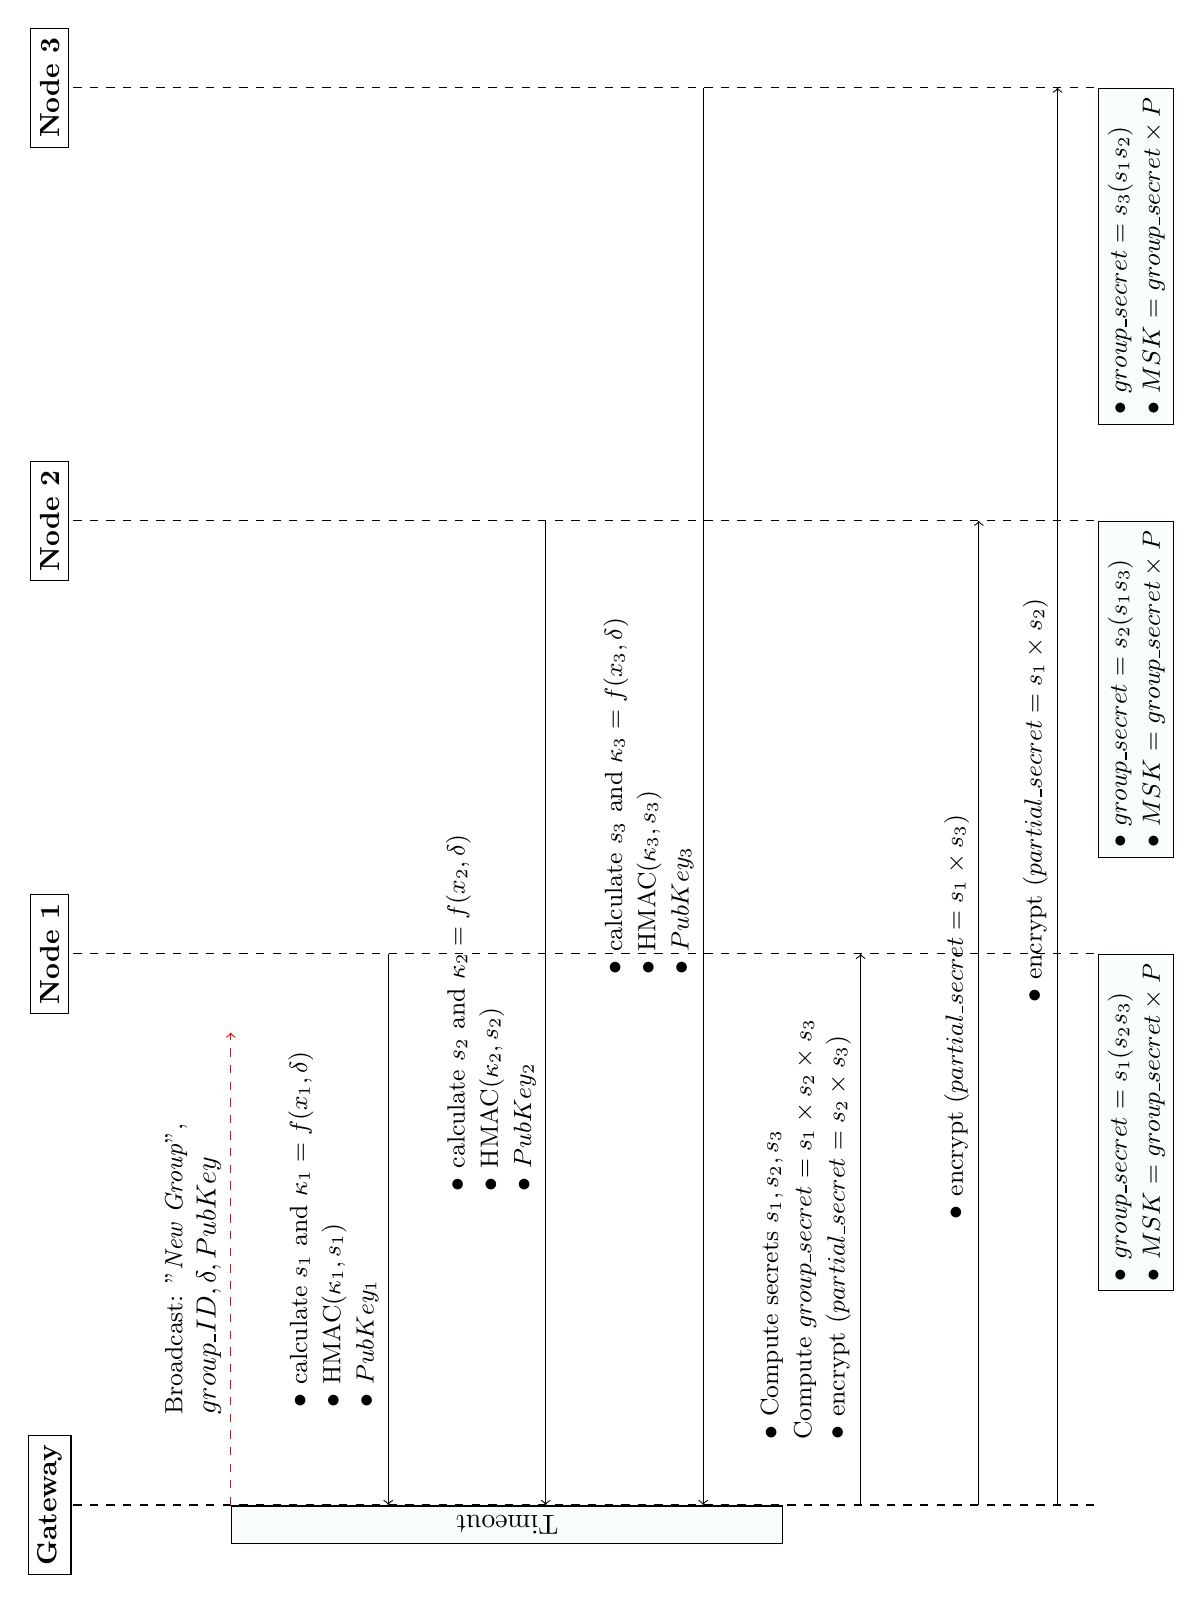
\begin{tikzpicture}[auto,rotate=90,transform shape]
    \draw (-8,0) -- (-8,-13)[dashed] (-1,0) -- (-1,-13)  (4.5,0) -- (4.5,-13)  (10,0) -- (10,-13);
    \node at (-8,.3) [draw,thin]{\textbf{Gateway}};
    \node at (-1,.3) [draw,thin]{\textbf{Node 1}};
    \node at (4.5,.3) [draw,thin]{\textbf{Node 2}};
    \node at (10,.3) [draw,thin]{\textbf{Node 3}};
    \node at (-8.25,-2) [drawrect, rotate=90, fill= SkyBlue!5, minimum width=7cm]  { Timeout};
    \draw[->, dashed, draw=red] (-8,-2) -- node[midway,above,align=left] {
        \small Broadcast: "\textit{New Group}",\\$group\_ID, \delta , PubKey$ 
        } (-2,-2);
    \draw[<-] (-8,-4) -- node[midway,above,align=left] {
    $\bullet$ \small calculate  $s_1$ and  $\kappa_1 = f(x_1,\delta)$\\
    $\bullet$ \small HMAC($\kappa_1 , s_1$)\\
    $\bullet$ \small $PubKey_1$
    } (-1,-4);
    
    \draw[<-] (-8,-6) -- node[midway,above,align=left] {
    $\bullet$ \small calculate  $s_2$ and  $\kappa_2 = f(x_2,\delta)$\\
    $\bullet$ \small HMAC($\kappa_2 , s_2$)\\
    $\bullet$ \small $PubKey_2$
    } (4.5,-6);
    
    \draw[<-] (-8,-8) -- node[midway,above,align=left] {
    $\bullet$ \small calculate  $s_3$ and  $\kappa_3 = f(x_3,\delta)$\\
    $\bullet$ \small HMAC($\kappa_3 , s_3$)\\
    $\bullet$ \small $PubKey_3$
    } (10,-8);
    
    \draw[->] (-8,-10) -- node[midway,above,align=left] {
    $\bullet$ \small Compute secrets $s_1, s_2, s_3$ \\
    \small Compute $group\_secret = s_1 \times s_2 \times s_3$ \\
    $\bullet$ \small encrypt ($partial\_secret = s_2 \times s_3$)
    } (-1,-10);
    
    \draw[->] (-8,-11.5) -- node[midway,above,align=left] {
    $\bullet$ \small encrypt ($partial\_secret = s_1 \times s_3$)
    } (4.5,-11.5);
    
    \draw[->] (-8,-12.5) -- node[midway,above,align=left] {
    $\bullet$ \small encrypt ($partial\_secret = s_1 \times s_2$)
    } (10,-12.5);
    
    \node at (-1,-13.5) [draw,thin, align=left, anchor=east, fill= SkyBlue!5 ]{
    \small $\bullet$ $group\_secret = s_1 (s_2 s_3)$\\
    \small$\bullet$ $MSK = group\_secret  \times \mathbb{P}$};
    
    \node at (4.5,-13.5) [draw,thin, align=left, anchor=east, fill= SkyBlue!5 ]{
    \small$\bullet$ $group\_secret = s_2 (s_1 s_3)$\\
    \small $\bullet$ $MSK = group\_secret  \times \mathbb{P}$};
    
    \node at (10,-13.5) [draw,thin, align=left, anchor=east, fill= SkyBlue!5 ]{
    \small$\bullet$ $group\_secret = s_3 (s_1 s_2)$\\
    \small$\bullet$ $MSK = group\_secret \times \mathbb{P}$};
\end{tikzpicture}
\end{center}
\caption{Group Key Initialization: The figure shows the messages exchanged between G and three end nodes which replied to the join request before the
specified timeout.}
\label{fig_group_key}
\end{figure*}

In this phase, a device that wants to start a secure group, usually the gateway, generates a unique $group\_ID$ and includes it in a "\textit{new\_group}" broadcasts message.
It also generate a public key $PubKey$ represented as a point on an elliptic curve and a couple of values $(\h(\kappa), \delta)$ through a commitment function $F$ using a context fingerprint as described in \ref{proxAuth}, including them in the broadcast message.

Now a specified timeout starts and the nodes that want to join the group reply to the broadcast message with their public key $PubKey_i$ in a \textit{JOIN} message. 
Each node calculate a secret $s_i$ shared with the gateway generated with Elliptic-curve Diffie-Hellman (\acs{ECDH}) protocol and , using a decommitment function $f$, extract from their context fingerprint $x_i$ the value $\kappa_i = f(x_i, \delta)$.
In the message, together with its public key, each node $i$ include the value $HMAC(\kappa_i, s_i)$, in order to guarantee confidentiality and authenticity.

The gateway \textit{G} collects the \textit{JOIN} replies until the timeout expires and then it calculates the secrets shared with each node $i$ willing to join the group and checks that $HMAC(\kappa , s_i) = HMAC(\kappa_i, s_i)$ in order to verify both integrity of the received message and that the node is located in the same ambient.
\textit{G} computes the $group\_secret = \prod_{i=1}^{m} s_{i}$ where $m$ is the number of nodes which replied to the $JOIN$ message and have been authenticated. \textit{G} finally sends to each node $n_i$ the value $partial\_secret = group\_secret / s_i$, encrypted with the shared secret using protocols such as AES.
This procedure is shown in Algorithm \ref{alg:init}.

\begin{algorithm}
\caption{Group-key initialization }\label{alg:init}
\hspace*{\algorithmicindent} \textbf{Input:} parameter $\mathbb{P}$ \\
\hspace*{\algorithmicindent} \textbf{Output:} \textit{group\_secret} \\
\hspace*{\algorithmicindent} \textbf{Initialization:} chose $group\_id, group\_secret = 1$, \\
\hspace*{\algorithmicindent} Broadcast group join request with {\textit{group\_id}, $\delta$, $PubKey$ }\\
\hspace*{\algorithmicindent} Set \textit{timeout}
\begin{algorithmic}[1]
\While{$timeout$ not expired}
\For{for each $JOIN_i$ message received} 
\State generate shared secret $s_i$
\If{$HMAC(\kappa, s_i) == HMAC(\kappa_i , s_i)$}
\State $group\_secret = group\_secret * s_i$
\EndIf
\EndFor{}
\EndWhile\label{secret}
\For{for each $s_i$ received and validated} 
\State $G \rightarrow n_i: \qquad E_{s_i}(group\_secret / s_i)$
\EndFor{}
\Return{$group\_secret$}
\end{algorithmic}
\end{algorithm}

After receiving the message, each node $n_i$ decrypts the message obtaining its own $partial\_secret$ and computes  
\begin{center}
$MSK = partial\_secret * s_i * \mathbb{P}$
\end{center}
where $MSK$ represents the group shared key.

\section{Join Procedure}
After establishing a secure $group\_secret$, the addition of a new node in the group may occur. 
When a new node $new\_node$ wants to join the group, it sends a message to $G$ containing the $group\_ID$ and its public key $PubKey$.
The gateway generate a couple of values $(\h(\kappa), \delta)$ through a commitment function $F$ using a fingerprint of its context and sending a \textit{challenge} to the $new\_node$ with a message containing $\delta$ and its own public key $PubKey$.
The new node replies to the the challenge with $HMAC(\kappa_n, s_n)$, where $\kappa_n$ is the secret key generated using a commitment function $F$ exploiting a context fingerprint.
At this point $G$ can verify that $new\_node$ is located in the same ambient and recomputes the $group\_secret$ as before including the secrets from the new nodes and broadcasting the $new\_MSK = group\_secret \times P$, encrypting the message with the previous $MSK$. 

In this phase we have to ensure that the new node isn't able to easily recover the old $MSK$. 
To solve this problem, $G$ picks a random secret $s_i$ from the nodes already present in the group  and sends to the $new\_node$ a message, encrypted with his shared secret $s_n$, containing $s_{i}\mathbb{P}$ and $partial\_secret = new\_group\_secret / s_i$.

\begin{algorithm}[H]
\caption{New node addition }\label{alg:newNode}
\hspace*{\algorithmicindent} \textbf{Input:} parameter $\mathbb{P}$ \\
\hspace*{\algorithmicindent} \textbf{Output:} \textit{group\_secret} \\
\hspace*{\algorithmicindent} \textbf{Initialization:} chose the \textit{group\_id} of the group to join,\\
\begin{algorithmic}[1]
\State $new\_node \rightarrow G:\qquad group\_ID, PubKey_n$
\State $G \rightarrow new\_node:\qquad \delta, PubKey$
\State $new\_node \rightarrow G:\qquad HMAC(\kappa_n, s_n)$
\If{$HMAC(\kappa_n, s_n) == HMAC(\kappa, s_n)$}
\State $old\_MSK = MSK$
\State $group\_secret = s_n * old\_group\_secret$
\For{for each node $n_i$ already in the group} 
\State $G \rightarrow n_i: \qquad E_{old\_MSK}( (MSK / s_i) \times \mathbb{P})$
\EndFor{}
\State $G$ picks a random $s_i$ of a node already in the group
\State $partial\_secret = group\_secret / s_i$
\State $G \rightarrow new\_node: \qquad E_{s_n}(s_{i}\mathbb{P}, partial\_secret)$
\State $new\_node$ calculates $MSK = s_{i}\mathbb{P} \times partial\_secret$\\
\EndIf
\Return{$group\_secret$}
\end{algorithmic}
\end{algorithm}

To obtain the $MSK$, the new node only has to multiply $s_{i}\mathbb{P}$ by $partial\_secret$ and it will not be able to recover the old $MSK$ due to difficulty to obtain $s_i$ from $s_{i}\mathbb{P}$.  %mention why it is difficult ? %
This procedure is shown in Algorithm \ref{alg:newNode}.

\section{Leave Procedure}

\begin{algorithm}[H]
\caption{Node removal's algorithm }\label{alg:remNode}
\hspace*{\algorithmicindent} \textbf{Input:} parameter $\mathbb{P}$ \\
\hspace*{\algorithmicindent} \textbf{Output:} \textit{group\_secret} \\
\hspace*{\algorithmicindent} \textbf{Initialization:} remove the node $n$ from the \\
\hspace*{\algorithmicindent} group $group\_id$\\
\begin{algorithmic}[1]
\State $G$ picks a random $s$ of a node in the group
\State $partial\_secret_i = group\_secret / (s_i s)$
\For{for each node $n_i$ already in the group} 
\State $G \rightarrow n_i: \qquad partial\_secret_i , s \mathbb{P}$
\EndFor{}

\State $n_i$ calculates $MSK = s \mathbb{P} * partial\_secret_i$\\
\Return{$group\_secret$}
\end{algorithmic}
\end{algorithm}

It can happen that one or more nodes have to be removed from the group for various reasons. In such an event, the protocol has to ensure forward secrecy of the $MSK$ to avoid the possibility that the removed node is able to get the new group secret. 
The gateway proceeds as described before picking up a random node's shared secret $s$ and sends to each node $n_i$ which belongs to the group a message containing a new partial secret $partial\_secret_i = group\_secret / (s_i s)$ and $s\mathbb{P}$. 
Each node can than compute $MSK$ by multiplying $partial\_secret_i$ by $s\mathbb{P}$ and its shared secret $s_i$. 
The nodes that have left the group will not be able to compute the new $MSK$ due to the same reason described during the \textit{node addition´s phase}.

\section{Generate Session Key}
After the $MSK$ generation, it is possible to use symmetric key encryption to encrypt the group messages. The choice of using symmetric key encryption instead of public key encryption is motivated by the fact that public key encryption is slower and requires more computation power, a critical point in this class of constrained IoT devices. 

Using the same key for more than one session makes the protocol vulnerable to many attacks \cite{Syverson}, so we generate new and pseudorandom keys from the $MSK$. The session key can be produced and managed in different ways depending on whether the encryption scheme is block or stream cipher. In this section we consider those two methods separately.  
$MSK$ with block ciphers: Suppose the block cipher of our
choice takes n-bit key size. Therefore, every session key must
be n-bit long. We assume we have a k-bit output hash function
h, and a $PRF$ that maps an input of l-bit key size to an output
of size $n$. Note that the output of the $PRF$ is computationally
indistinguishable from an output of a random function from
l to n. An l-bit input seed to our $PRF$ is first formed by
concatenating the results of a repeated application of a hash
function applied to a nonce and $MSK$, as shown below.
\begin{center}
$seed = h(nonce_1 \parallel MSK) \parallel h(nonce_2 \parallel MSK) \parallel \cdots$
\end{center}
A session key is then generated by feeding the seed into a
$PRF$.
\begin{center}
$session\_key = PRF(seed)$
\end{center}
And finally $MSK$ is updated to the new session key. 
Note that the node sending a group message randomly selects as many nonce values as needed to create an l-bit output. 
The nonce values are sent in the clear to all nodes so that every nodes updates its session key similarly.

$MSK$ with stream ciphers: in this case, it is required tha twe produce a session key as long as the length of the text
to be encrypted. This can be achieved by concatenating the
results of the $PRF$ on many seed values as follows.
\begin{center}
$seed 1 = h(nonce_1 \parallel MSK)$\\
$seed_2= h(nonce_2 \parallel MSK)$\\
$\vdots$ \\
$seed_n = h(nonce_n \parallel MSK)$
\end{center}

We then apply the $PRF$ to each seed seed and simply
concatenate the results to generate a session key as long as
required.
\begin{center}
$session\_key = PRF (seed_1) || PRF (seed_2) || \cdot$
\end{center}
In both cases, encryption is done as follows :
\begin{center}
$Encrypt(M) = f(M, Session key)$
\end{center}
Where $f$ could by any block cipher, such as AES, or stream
cipher, such as RC4.

